\let\negmedspace\undefined
\let\negthickspace\undefined
\documentclass[journal,12pt,onecolumn]{article}
\usepackage{cite}
\usepackage{amsmath,amssymb,amsfonts,amsthm}
\usepackage{algorithmic}
\usepackage{graphicx}
\usepackage{textcomp}
\usepackage{xcolor}
\usepackage{txfonts}
\usepackage{listings}
\usepackage{enumitem}
\usepackage{mathtools}
\usepackage{gensymb}
\usepackage{comment}
\usepackage[breaklinks=true]{hyperref}
\usepackage{tkz-euclide} 
\usepackage{listings}
\usepackage{gvv}                                        
%\def\inputGnumericTable{}                                 
\usepackage[latin1]{inputenc}     
\usepackage{xparse}
\usepackage{color}                                            
\usepackage{array}                                            
\usepackage{longtable}                                       
\usepackage{calc}                                             
\usepackage{multirow}
\usepackage{multicol}
\usepackage{hhline}                                           
\usepackage{ifthen}                                           
\usepackage{lscape}
\usepackage{tabularx}
\usepackage{array}
\usepackage{float}
\usepackage{bm}
\newtheorem{theorem}{Theorem}[section]
\newtheorem{problem}{Problem}
\newtheorem{proposition}{Proposition}[section]
\newtheorem{lemma}{Lemma}[section]
\newtheorem{corollary}[theorem]{Corollary}
\newtheorem{example}{Example}[section]
\newtheorem{definition}[problem]{Definition}
\newcommand{\BEQA}{\begin{eqnarray}}
\newcommand{\EEQA}{\end{eqnarray}}
\usepackage{float}
%\newcommand{\define}{\stackrel{\triangle}{=}}
\theoremstyle{remark}
\usepackage{ circuitikz }
%\newtheorem{rem}{Remark}
% Marks the beginning of the document
\begin{document}

\title{CE - 2009}
\author{EE25BTECH11043 - Nishid Khandagre}
\date{}
\maketitle

\renewcommand{\thefigure}{\theenumi}
\renewcommand{\thetable}{\theenumi}


\section*{Q. 1 - Q. 20 carry one mark each.}
\begin{enumerate}
    \item A square matrix B is skew-symmetric if (GATE-CE 2009)
    \begin{multicols}{2}
    \begin{enumerate}
        \item $\vec{B}^T = -\vec{B}$ 
        \item $\vec{B}^T = \vec{B}$ 
        \item $\vec{B}^{-1} = \vec{B}$ 
        \item $\vec{B}^{-1} = \vec{B}^T$
    \end{enumerate}
    \end{multicols}
    
    \item For a scalar function $f(x, y, z) = x^2 + 3y^2 + 2z^2$, the gradient at the point P (1, 2, -1) is (GATE-CE 2009)
    \begin{multicols}{2}
    \begin{enumerate}
        \item $2\hat{i} + 6\hat{j}+ 4\hat{k}$
        \item $2\hat{i} + 12\hat{j} - 4\hat{k}$
        \item $2\hat{i} + 12\hat{j} + 4\hat{k}$
        \item $\sqrt{56}$
    \end{enumerate}
    \end{multicols}
    
    \item The analytic function
\begin{align}
f(z) &= \frac{z-1}{z^2+1}
\end{align}
has singularities at (GATE-CE 2009)
    \begin{multicols}{2}
    \begin{enumerate}
        \item 1 and -1 
        \item 1 and i 
        \item 1 and -i 
        \item i and -i
    \end{enumerate}
    \end{multicols}
    
    \item A thin walled cylindrical pressure vessel having a radius of 0.5 m and wall thickness of 25 mm is subjected to an internal pressure of 700 kPa. The hoop stress developed is (GATE-CE 2009)
    \begin{multicols}{2}
    \begin{enumerate}
        \item 14 MPa 
        \item 1.4 MPa 
        \item 0.14 MPa 
        \item 0.014 MPa
    \end{enumerate}
    \end{multicols}
    
    \item The modulus of rupture of concrete in terms of its characteristic cube compressive strength ($f_{ck}$) in MPa according to IS 456:2000 is (GATE-CE 2009)
    \begin{multicols}{2}
    \begin{enumerate}
        \item $5000f_{ck}$ 
        \item $0.7f_{ck}$ 
        \item $5000\sqrt{f_{ck}}$ 
        \item $0.7\sqrt{f_{ck}}$
    \end{enumerate}
    \end{multicols}
    
    \item In the theory of plastic bending of beams, the ratio of plastic moment to yield moment is called (GATE-CE 2009)
    \begin{multicols}{2}
    \begin{enumerate}
        \item shape factor 
        \item plastic section modulus 
        \item modulus of resilience 
        \item rigidity modulus
    \end{enumerate}
    \end{multicols}
    
    \item For limit state of collapse, the partial safety factors recommended by IS 456:2000 for estimating the design strength of concrete and reinforcing steel are respectively (GATE-CE 2009)
    \begin{multicols}{2}
    \begin{enumerate}
        \item 1.15 and 1.5 
        \item 1.0 and 1.0 
        \item 1.5 and 1.15 
        \item 1.5 and 1.0
    \end{enumerate}
    \end{multicols}
    
    \item The point within the cross sectional plane of a beam through which the resultant of the external loading on the beam has to pass through to ensure pure bending without twisting of the cross-section of the beam is called (GATE-CE 2009)
    \begin{multicols}{2}
    \begin{enumerate}
        \item moment centre 
        \item centroid 
        \item shear centre 
        \item elastic center
    \end{enumerate}
    \end{multicols}
    
    \item The square root of the ratio of moment of inertia of the cross section to its cross sectional area is called (GATE-CE 2009)
    \begin{multicols}{2}
    \begin{enumerate}
        \item second moment of area 
        \item slenderness ratio 
        \item section modulus 
        \item radius of gyration
    \end{enumerate}
    \end{multicols}
    
    \item Deposit with flocculated structure is formed when (GATE-CE 2009)
    \begin{enumerate}
        \item clay particles settle on sea bed 
        \item clay particles settle on fresh water lake bed 
        \item sand particles settle on river bed 
        \item sand particles settle on sea bed
    \end{enumerate}
    
    \item Dilatancy correction is required when a strata is (GATE-CE 2009)
    \begin{enumerate}
        \item cohesive and saturated and also has N value of SPT $>$ 15
        \item saturated silt/fine sand and N value of SPT $<$10 after the overburden correction
        \item saturated silt/fine sand and N value of SPT $>$15 after the overburden correction
        \item coarse sand under dry condition and N value of SPT $<$10 after the overburden correction
    \end{enumerate}
    
    \item A precast concrete pile is driven with a 50 kN hammer falling through a height of 1.0 m with an efficiency of 0.6. The set value observed is 4 mm per blow and the combined temporary compression of the pile, cushion and the ground is 6 mm. As per Modified Hiley Formula, the ultimate resistance of the pile is (GATE-CE 2009)
    \begin{multicols}{2}
    \begin{enumerate}
        \item 3000 kN 
        \item 4285.7 kN 
        \item 8333 kN 
        \item 11905 kN
    \end{enumerate}
    \end{multicols}
    
    \item Direct step method of computation for gradually varied flow is (GATE-CE 2009)
    \begin{enumerate}
        \item applicable to non-prismatic channels
        \item applicable to prismatic channels
        \item applicable to both prismatic and non-prismatic channels
        \item not applicable to both prismatic and non-prismatic channels
    \end{enumerate}
    
    \item The relationship among specific yield ($S_y$), specific retention ($S_r$) and porosity ($\eta$) of an aquifer is (GATE-CE 2009)
    \begin{multicols}{2}
    \begin{enumerate}
        \item $S_y = S_r + \eta$ 
         \item $S_y = S_r - \eta$ 
        \item $S_y = \eta - S_r$ 
        \item $S_y = S_r + 2\eta$
    \end{enumerate}
    \end{multicols}
    
    \item The depth of flow in an alluvial channel is 1.5 m. If critical velocity ratio is 1.1 and Manning's n is 0.018, the critical velocity of the channel as per Kennedy's method is (GATE-CE 2009)
    \begin{multicols}{2}
    \begin{enumerate}
        \item $0.713~\mathrm{m/s}$
        \item $0.784~\mathrm{m/s}$
        \item $0.879~\mathrm{m/s}$
        \item $1.108~\mathrm{m/s}$
    \end{enumerate}
    \end{multicols}
    
    \item The reference pressure used in the determination of sound pressure level is (GATE-CE 2009)
    \begin{multicols}{2}
    \begin{enumerate}
        \item $20~\mu\mathrm{Pa}$
        \item $20~\mathrm{db}$
        \item $10~\mu\mathrm{Pa}$
        \item $10~\mathrm{db}$
    \end{enumerate}
    \end{multicols}
    
    \item Particulate matter (fly ash) carried in effluent gases from the furnaces burning fossil fuels are better removed by (GATE-CE 2009)
    \begin{enumerate}
        \item Cotton bag house filter 
        \item Electrostatic precipitator (ESP)
        \item Cyclone 
        \item Wet scrubber
    \end{enumerate}
    
    \item The value of lateral friction or side friction used in the design of horizontal curve as per Indian Roads Congress guidelines is (GATE-CE 2009)
    \begin{multicols}{4}
    \begin{enumerate}
        \item 0.40 
        \item 0.35 
        \item 0.24 
        \item 0.15
    \end{enumerate}
    \end{multicols}
    
    \item During a CBR test, the load sustained by a remolded soil specimen at 5.0 mm penetration is 50 kg. The CBR value of the soil will be (GATE-CE 2009)
    \begin{multicols}{2}
    \begin{enumerate}
        \item 10.0 \% 
        \item 5.0 \% 
        \item 3.6 \% 
        \item 2.4 \%
    \end{enumerate}
    \end{multicols}
    
    \item In quadrantal bearing system, bearing of a line varies from (GATE-CE 2009)
    \begin{multicols}{2}
    \begin{enumerate}
        \item $0\degree$ to $360\degree$ 
        \item $0\degree$ to $180\degree$
        \item $0\degree$ to $90\degree$ 
        \item $0\degree$ N to $90\degree$ S
    \end{enumerate}
    \end{multicols}

\section*{Q. 21 to Q. 60 carry two marks each.}

    \item For a scalar function $f(x, y, z) = x^2 + 3y^2 + 2z^2$, the directional derivative at the point P (1, 2, -1) in the direction of a vector $\hat{i} - \hat{j} + 2\hat{k}$ is (GATE-CE 2009)
    \begin{multicols}{4}
    \begin{enumerate}
        \item -18 
        \item $-3\sqrt{6}$ 
        \item $3\sqrt{6}$ 
        \item 18
    \end{enumerate}
    \end{multicols}

    \item The value of the integral $\int_{c} \frac{\cos(2\pi z)}{(2z-1)(z-3)} dz$ (where c is a closed curve given by $|z|=1$) is (GATE-CE 2009)
    \begin{multicols}{2}
    \begin{enumerate}
        \item $-\pi i$ 
        \item $\frac{\pi i}{5}$ 
        \item $\frac{2\pi i}{5}$ 
        \item $\pi i$
    \end{enumerate}
    \end{multicols}
    
    \item Solution of the differential equation $3y\frac{dy}{dx}+2x=0$ represents a family of (GATE-CE 2009)
    \begin{multicols}{2}
    \begin{enumerate}
        \item ellipses 
        \item circles 
        \item parabolas 
        \item hyperbolas
    \end{enumerate}
    \end{multicols}
    
    \item Laplace transform for the function $f(x)=\cosh(ax)$ is (GATE-CE 2009)
    \begin{multicols}{2}
    \begin{enumerate}
        \item $\frac{a}{s^2-a^2}$ 
        \item $\frac{s}{s^2-a^2}$ 
        \item $\frac{a}{s^2+a^2}$ 
        \item $\frac{s}{s^2+a^2}$
    \end{enumerate}
    \end{multicols}
    
    \item In the solution of the following set of linear equations by Gauss elimination using partial pivoting  
    $5x+y+2z=34$;  $4y-3z=12$; and  $10x-2y+z=-4$; 
    the pivots for elimination of x and y are (GATE-CE 2009)
    \begin{multicols}{2}
    \begin{enumerate}
        \item 10 and 4 
        \item 10 and 2 
        \item 5 and 4 
        \item 5 and -4
    \end{enumerate}
    \end{multicols}
    
    \item The standard normal probability function can be approximated as
    \[ F(x_N) = \frac{1}{1+\exp\left(-1.7255 x_N | x_N |^{0.12}\right)} \]
    where $x_N$ = standard normal deviate. If mean and standard deviation of annual precipitation are 102 cm and 27 cm respectively, the probability that the annual precipitation will be between 90 cm and 102 cm is (GATE-CE 2009)
    \begin{multicols}{2}
    \begin{enumerate}
        \item 66.7 \% 
        \item 50.0 \% 
        \item 33.3 \% 
        \item 16.7 \%
    \end{enumerate}
    \end{multicols}
    
    \item Consider the following statements: (GATE-CE 2009)
    \begin{itemize}
        \item[I.] On a principal plane, only normal stress acts.
        \item[II.] On a principal plane, both normal and shear stresses act.
        \item[III.] On a principal plane, only shear stress acts.
        \item[IV.] Isotropic state of stress is independent of frame of reference.
    \end{itemize}
    The TRUE statements are
    \begin{multicols}{2}
    \begin{enumerate}
        \item I and IV 
        \item II 
        \item II and IV 
        \item II and III
    \end{enumerate}
\end{multicols}
    
    \item The degree of static indeterminacy of a rigidly jointed frame in a horizontal plane and subjected to vertical loads only, as shown in figure below, is (GATE-CE 2009)
    \begin{figure}[H]
    \centering
    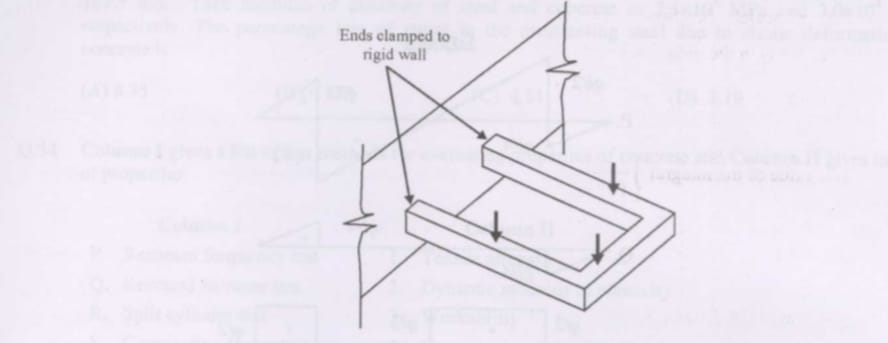
\includegraphics[width=0.7\columnwidth]{figs/image.jpg}
    \caption{}
    \label{fig:placeholder}
    \end{figure}
    \begin{multicols}{4}
    \begin{enumerate}
        \item 6 
        \item 4 
        \item 3 
        \item 1
    \end{enumerate}
\end{multicols}
    
    \item A 12 mm thick plate is connected to two 8 mm thick plates, on either side through a 16 mm diameter power driven field rivet as shown in the figure below. Assuming permissible shear stress as 90 MPa and permissible bearing stress as 270 MPa in the rivet, the rivet value of the joint is (GATE-CE 2009)
    \begin{figure}[H]
    \centering
    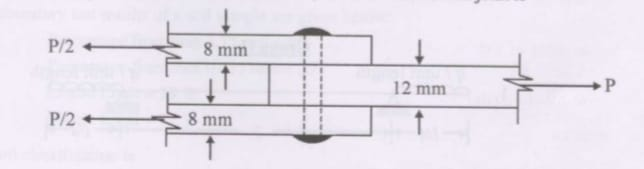
\includegraphics[width=0.7\columnwidth]{figs/image2.jpg}
    \caption{}
    \label{fig:placeholder}
    \end{figure}
    
    \begin{multicols}{2}
    \begin{enumerate}
        \item 56.70 kN 
        \item 43.29 kN
        \item 36.19 kN 
        \item 21.65 kN
    \end{enumerate}
\end{multicols}
    
    \item A hollow circular shaft has an outer diameter of 100 mm and a wall thickness of 25 mm. The allowable shear stress in the shaft is 125 MPa. The maximum torque the shaft can transmit is (GATE-CE 2009)
    \begin{multicols}{2}
    \begin{enumerate}
        \item 46 kN m 
        \item 24.5 kN m 
        \item 23 kN m 
        \item 11.5 kN m
    \end{enumerate}
\end{multicols}
    
    \item Consider the following statements for a compression member: (GATE-CE 2009)
    \begin{itemize}
        \item[I.] The elastic critical stress in compression increases with decrease in slenderness ratio.
        \item[II.] The effective length depends on the boundary conditions at its ends.
        \item[III.] The elastic critical stress in compression is independent of the slenderness ratio.
        \item[IV.] The ratio of the effective length to its radius of gyration is called as slenderness ratio.
    \end{itemize}
    The TRUE statements are \\
    \begin{multicols}{2}
    \begin{enumerate}
        \item II and III 
        \item III and IV 
        \item II, III and IV 
        \item I, II and IV
    \end{enumerate}
\end{multicols}
    
    \item Group I gives the shear force diagrams and Group II gives the diagrams of beams with supports and loading. Match the Group I with Group II. (GATE-CE 2009)

    \begin{figure}[H]
        \centering
        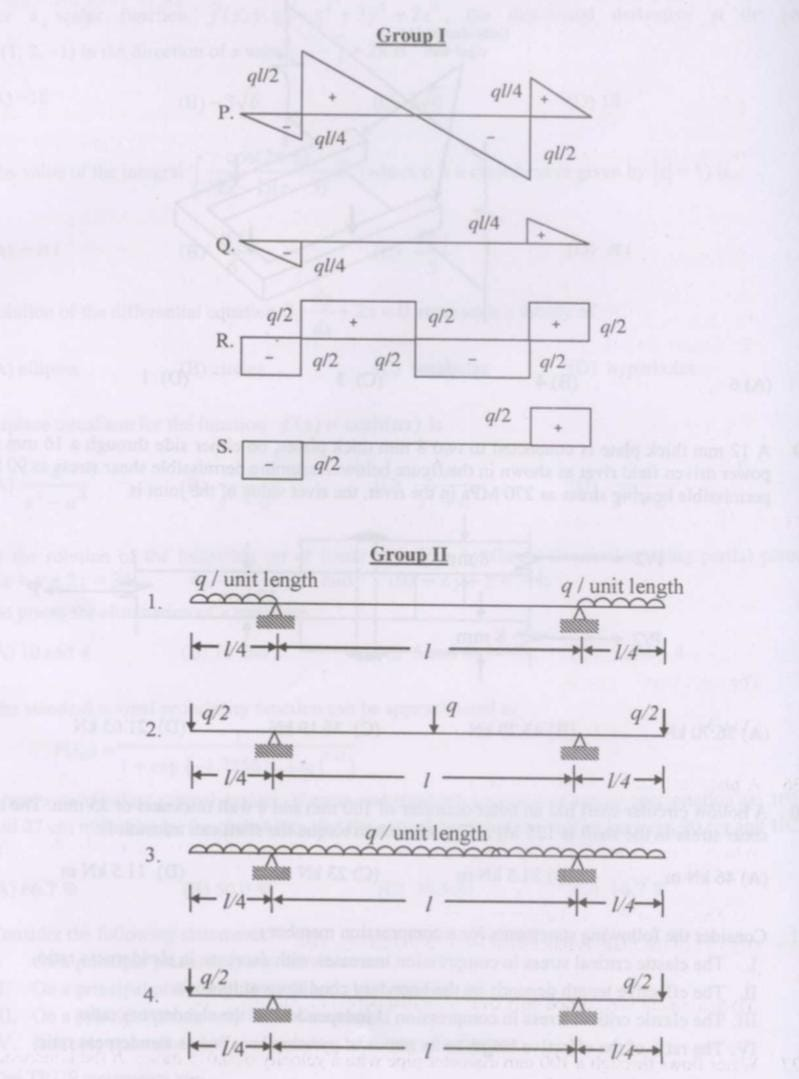
\includegraphics[width=0.7\columnwidth]{figs/image3.jpg}
        \caption{}
        \label{fig:placeholder}
    \end{figure}
    
    \begin{enumerate}
        \item P-3, Q-1, R-2, S-4 
        \item P-3, Q-4, R-2, S-1 
        \item P-2, Q-1, R-4, S-3 
        \item P-2, Q-4, R-3, S-4
    \end{enumerate}
    
    \item A rectangular concrete beam of width 120 mm and depth 200 mm is prestressed by pretensioning to a force of 150 kN at an eccentricity of 20 mm. The cross sectional area of the prestressing steel is 187.5 mm$^2$. Take modulus of elasticity of steel and concrete as $2.1 \times 10^5\, \text{MPa}$ and $3.0 \times 10^4\, \text{MPa}$ respectively. The percentage loss of stress in the prestressing steel due to elastic deformation of concrete is (GATE-CE 2009)
    \begin{multicols}{2}
    \begin{enumerate}
        \item 8.75 
        \item 6.125 
        \item 4.81 
        \item 2.19
    \end{enumerate}
\end{multicols}
    
    \item Column I gives a list of test methods for evaluating properties of concrete and Column II gives the list of properties. (GATE-CE 2009)
    \begin{center}
    \begin{tabular}{|l|l|}
    \hline
    \textbf{Column I} & \textbf{Column II} \\
    \hline
    P. Resonant frequency test & 1. Tensile strength \\
    Q. Rebound hammer test & 2. Dynamic modulus of elasticity \\
    R. Split cylinder test & 3. Workability \\
    S. Compacting factor test & 4. Compressive strength \\
    \hline
    \end{tabular}
    \end{center}
    The correct match of the test with the property is
    \begin{enumerate}
        \item P-2, Q-4, R-1, S-3 
        \item P-2, Q-1, R-4, S-3 
        \item P-2, Q-4, R-3, S-1 
        \item P-4, Q-3, R-1, S-2
    \end{enumerate}
    
    \item The laboratory test results of a soil sample are given below: (GATE-CE 2009)
    \begin{itemize}
        \item Percentage finer than 4.75 mm = 60
        \item Percentage finer than 0.075 mm = 30
        \item Liquid Limit = 35 \%
        \item Plastic Limit = 27 \%
    \end{itemize}
    The soil classification is
    \begin{multicols}{4}
    \begin{enumerate}
        \item GM 
        \item SM 
        \item GC 
        \item ML--MI
    \end{enumerate}
\end{multicols}
    
    \item A plate load test is carried out on a 300 mm $\times$ 300 mm plate placed at 2 m below the ground level to determine the bearing capacity of a 2 m $\times$ 2 m footing placed at same depth of 2 m on a homogeneous sand deposit extending 10 m below ground. The ground water table is 3 m below the ground level. Which of the following factors does not require a correction to the bearing capacity determined based on the load test? (GATE-CE 2009)
    \begin{enumerate}
        \item Absence of the overburden pressure during the test
        \item Size of the plate is much smaller than the footing size
        \item Influence of the ground water table
        \item Settlement is recorded only over a limited period of one or two days
    \end{enumerate}
    
    \item Water flows through a 100 mm diameter pipe with a velocity of 0.015 m/sec. If the kinematic viscosity of water is 1.13$\times$10$^{-6}$ m$^2$/sec, the friction factor of the pipe material is (GATE-CE 2009)
    \begin{multicols}{4}
    \begin{enumerate}
        \item 0.0015 
        \item 0.032 
        \item 0.037 
        \item 0.048
    \end{enumerate}
\end{multicols}
    
    \item A rectangular open channel of width 4.5 m is carrying a discharge of 100 m$^3$/sec. The critical depth of the channel is (GATE-CE 2009)
    \begin{multicols}{2}
    \begin{enumerate}
        \item 7.09 m 
        \item 3.69 m 
        \item 2.16 m 
        \item 1.31 m
    \end{enumerate}
\end{multicols}
    
    \item Water ($\gamma_w = 9.879 \text{kN/m}^3$) flows with a flow rate of 0.3 m$^3$/sec through a pipe AB of 10 m length and of uniform cross section. The end 'B' is above end 'A' and the pipe makes an angle of $30\degree$ to the horizontal. For a pressure of 12 kN/m$^2$ at the end 'B', the corresponding pressure at the end 'A' is (GATE-CE 2009)
   \begin{multicols}{2}
    \begin{enumerate}
        \item 12.0 kN/m$^2$ 
        \item 17.0 kN/m$^2$ 
        \item 56.4 kN/m$^2$ 
        \item 61.4 kN/m$^2$
    \end{enumerate}
\end{multicols}
    
    \item An agricultural land of 437 ha is to be irrigated for a particular crop. The base period of the crop is 90 days and the total depth of water required by the crop is 105 cm. If a rainfall of 15 cm occurs during the base period, the duty of irrigation water is (GATE-CE 2009)
    \begin{multicols}{2}
    \begin{enumerate}
        \item 437 ha/cumec 
        \item 486 ha/cumec 
        \item 741 ha/cumec 
        \item 864 ha/cumec
    \end{enumerate}
\end{multicols}

    \item Match Column I with Column II: (GATE-CE 2009)
    \begin{center}
    \begin{tabular}{|l|l|}
    \hline
    \textbf{Column I} & \textbf{Column II} \\
    \hline
    P. Coriolis effect & 1. Rotation of earth \\
    Q. Fumigation & 2. Lapse rate and vertical temperature profile \\
    R. Ozone layer & 3. Inversion \\
    S. Maximum mixing depth(mixing height) & 4. Dobson \\
    \hline
    \end{tabular}
    \end{center}
    The correct match of Column I with Column II is
    \begin{enumerate}
        \item P-2, Q-1, R-4, S-3 
        \item P-2, Q-1, R-3, S-4 
        \item P-1, Q-3, R-2, S-4 
        \item P-1, Q-3, R-4, S-2
    \end{enumerate}
    
    \item A horizontal flow primary clarifier treats wastewater in which 10\%, 60\% and 30\% of particles have settling velocities of 0.1 mm/s, 0.2 mm/s, and 1.0 mm/s respectively. What would be the total percentage of particles removed if clarifier operates at a Surface Overflow Rate (SOR) of 43.2 m$^3$/m$^2$.d? (GATE-CE 2009)
   \begin{multicols}{4}
    \begin{enumerate}
        \item 43 \% 
        \item 56 \% 
        \item 86 \% 
        \item 100 \%
    \end{enumerate}
\end{multicols}
    
    \item An aerobic reactor receives wastewater at a flow rate of 500 m$^3$/d having a COD of 2000 mg/L. The effluent COD is 400 mg/L. Assuming that wastewater contains 80\% biodegradable waste, the daily volume of methane produced by the reactor is (GATE-CE 2009)
    \begin{multicols}{2}
    \begin{enumerate}
        \item 0.224 m$^3$ 
        \item 0.280 m$^3$ 
        \item 224 m$^3$ 
        \item 280 m$^3$
    \end{enumerate}
\end{multicols}
    
    \item Match Column I with Column II: (GATE-CE 2009)
    \begin{center}
    \begin{tabular}{|l|l|}
    \hline
    \textbf{Column I} & \textbf{Column II} \\
    \hline
    P. Grit chamber & 1. Zone settling \\
    Q. Secondary settling tank & 2. Stoke's law \\
    R. Activated sludge process & 3. Aerobic \\
    S. Trickling filter & 4. Contact stabilisation \\
    \hline
    \end{tabular}
    \end{center}
    The correct match of Column I with Column II is
    \begin{enumerate}
        \item P-1, Q-2, R-3, S-4 
        \item P-2, Q-1, R-3, S-4 
        \item P-1, Q-2, R-4, S-3 
        \item P-2, Q-1, R-4, S-3
    \end{enumerate}
    
    \item Which of the following stress combinations are appropriate in identifying the critical condition for the design of concrete pavements? (GATE-CE 2009)
    \begin{center}
    \begin{tabular}{|l|l|}
    \hline
    \textbf{Type of Stress} & \textbf{Location} \\
    \hline
    P. Load & 1. Corner \\
    Q. Temperature & 2. Edge \\
    & 3. Interior \\
    \hline
    \end{tabular}
    \end{center}
    \begin{multicols}{2}
    \begin{enumerate}
        \item P-2, Q-3 
        \item P-1, Q-3 
        \item P-3, Q-1 
        \item P-2, Q-2
    \end{enumerate}
\end{multicols}
    
    \item A crest vertical curve joins two gradients of +3\% and -2\% for a design speed of 80 km/h and the corresponding stopping sight distance of 120 m. The height of driver's eye and the object above the road surface are 1.20 m and 0.15 m respectively. The curve length (which is less than stopping sight distance) to be provided is (GATE-CE 2009)
    \begin{multicols}{4}
    \begin{enumerate}
        \item 120 m 
        \item 152 m 
        \item 163 m 
        \item 240 m
    \end{enumerate}
\end{multicols}
    
    \item On a specific highway, the speed-density relationship follows the Greenberg's model $[v = v_f \ln(k_j / k)]$, where $v_f$ and $k_j$ are the free flow speed and jam density respectively. When the highway is operating at capacity, the density obtained as per this model is (GATE-CE 2009)
    \begin{multicols}{2}
    \begin{enumerate}
        \item e.$k_j$ 
        \item $k_j$ 
        \item $k_j$/2 
        \item $k_j$/e
    \end{enumerate}
\end{multicols}
    
    \item A three-phase traffic signal at an intersection is designed for flows shown in the figure below. There are six groups of flows identified by the numbers 1 through 6. Among these 1, 3, 4, and 6 are through flows and, 2 and 5 are right turning. Which phasing scheme is not feasible? (GATE-CE 2009)
    \begin{figure}[H]
    \centering
    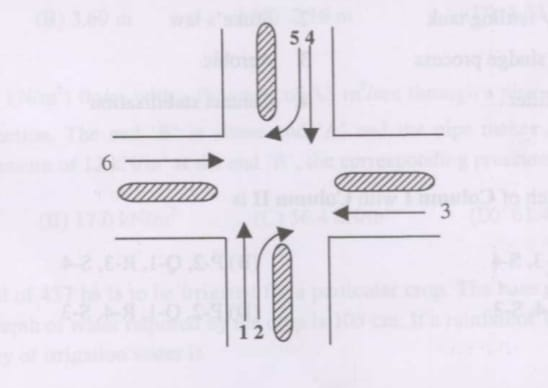
\includegraphics[width=0.7\columnwidth]{figs/image4.jpg}
    \caption{}
    \label{fig:placeholder}
    \end{figure}
    \begin{tabular}{|c|c|c|c|}
    \hline
    Combination choice & Phase I & Phase II & Phase III \\
    \hline
    P & 1, 4 & 2, 5 & 3, 6 \\
    Q & 1, 2 & 4, 5 & 3, 6 \\
    R & 2, 5 & 1, 3 & 4, 6 \\
    S & 1, 4 & 2, 6 & 3, 5 \\
    \hline
    \end{tabular}
    \begin{multicols}{4}
    \begin{enumerate}
        \item P 
        \item Q 
        \item R 
        \item S
    \end{enumerate}
\end{multicols}
    
    \item The magnetic bearing of a line AB was N $59\degree$ 30' W in the year 1967, when the declination was $4\degree$ 10' E. If the present declination is $3\degree$ W, the whole circle bearing of the line is (GATE-CE 2009)
    \begin{multicols}{2}
    \begin{enumerate}
        \item $299\degree$ 20' 
        \item $307\degree$ 40' 
        \item $293\degree$ 20' 
        \item $301\degree$ 40'
    \end{enumerate}
\end{multicols}
    
    \item Determine the correctness or otherwise of the following Assertion [a] and the Reason [r]: (GATE-CE 2009)

    \textbf{Assertion [a]}: Curvature correction must be applied when the sights are long.

    \textbf{Reason [r]}: Line of collimation is not a level line but is tangential to the level line.
    \begin{enumerate}
        \item Both [a] and [r] are true and [r] is the correct reason for [a].
        \item Both [a] and [r] are true but [r] is not the correct reason for [a].
        \item Both [a] and [r] are false.
        \item The [a] is false but [r] is true.
    \end{enumerate}

\section*{Common Data Questions}
\textbf{Common Data for Questions 51 and 52:}

Examine the test arrangement and the soil properties given below:
\begin{figure}[H]
    \centering
    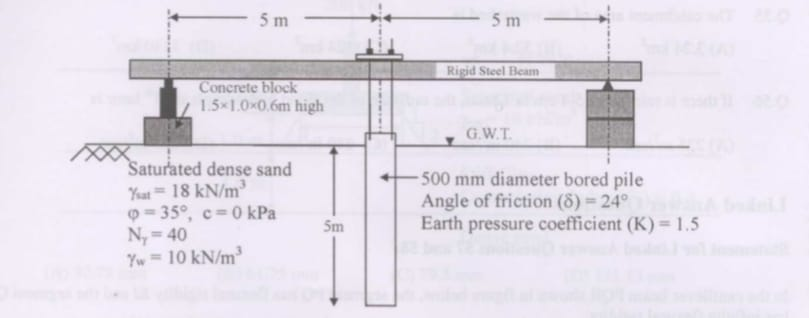
\includegraphics[width=0.7\columnwidth]{figs/image5.jpg}
    \caption{}
    \label{fig:placeholder}
    \end{figure}

    \item The maximum pressure that can be applied with a factor of safety of 3 through the concrete block, ensuring no bearing capacity failure in soil using Terzaghi's bearing capacity equation without considering the shape factor, depth factor and inclination factor is (GATE-CE 2009)
    \begin{multicols}{2}
    \begin{enumerate}
        \item 26.67 kPa 
        \item 60 kPa 
        \item 90 kPa 
        \item 120 kPa
    \end{enumerate}
\end{multicols}
    
    \item The maximum resistance offered by the soil through skin friction while pulling out the pile from the ground is (GATE-CE 2009)
    \begin{multicols}{4}
    \begin{enumerate}
        \item 104.9 kN 
        \item 209.8 kN 
        \item 236 kN 
        \item 472 kN
    \end{enumerate}
\end{multicols}

\textbf{Common Data for Questions 53 and 54:}

Following chemical species were reported for water sample from a well:
\begin{center}
\begin{tabular}{|l|c|}
\hline
\textbf{Species} & \textbf{Concentration (milli equivalent/L)} \\
\hline
Chloride (Cl$^-$) & 15 \\
Sulphate (SO$_4^{2-}$) & 15 \\
Carbonate (CO$_3^{2-}$) & 5 \\
Bicarbonate (HCO$_3^-$) & 30 \\
Calcium (Ca$^{2+}$) & 12 \\
Magnesium (Mg$^{2+}$) & 18 \\
pH & 8.5 \\
\hline
\end{tabular}
\end{center}

    \item Total hardness in mg/L as CaCO$_3$ is (GATE-CE 2009)
    \begin{multicols}{2}
    \begin{enumerate}
        \item 1500 
        \item 2000 
        \item 3000 
        \item 5000
    \end{enumerate}
\end{multicols}
    
    \item Alkalinity present in the water in mg/L as CaCO$_3$ is (GATE-CE 2009)
    \begin{multicols}{4}
    \begin{enumerate}
        \item 250 
        \item 1500 
        \item 1750 
        \item 5000
    \end{enumerate}
\end{multicols}

\textbf{Common Data for Questions 55 and 56:}

One hour triangular unit hydrograph of a watershed has the peak discharge of 60~m$^3$/sec.cm at 10 hours and time base of 30 hours. The $\phi$ index is 0.4 cm per hour and base flow is 15 m$^3$/sec.

    \item The catchment area of the watershed is (GATE-CE 2009)
    \begin{multicols}{2}
    \begin{enumerate}
        \item 3.24 km$^2$ 
        \item 32.4 km$^2$ 
        \item 324 km$^2$ 
        \item 3240 km$^2$
    \end{enumerate}
\end{multicols}
    
    \item If there is rainfall of 5.4 cm in 1 hour, the ordinate of the flood hydrograph at 15$^\text{th}$ hour is (GATE-CE 2009)
    \begin{multicols}{2}
    \begin{enumerate}
        \item 225~m$^3$/sec 
        \item 240~m$^3$/sec 
        \item 249~m$^3$/sec 
        \item 258~m$^3$/sec
    \end{enumerate}
\end{multicols}

\section*{Linked Answer Questions}
\textbf{Statement for Linked Answer Questions 57 and 58:}

In the cantilever beam PQR shown in figure below, the segment PQ has flexural rigidity EI and the segment QR has infinite flexural rigidity
    \begin{figure}[H]
    \centering
    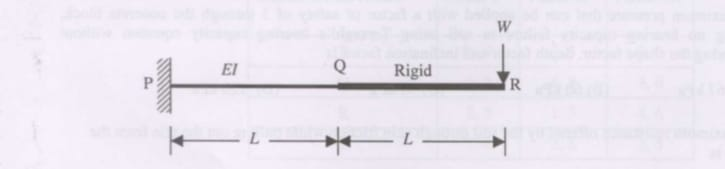
\includegraphics[width=0.7\columnwidth]{figs/image6.jpg}
    \caption{}
    \label{fig:placeholder}
    \end{figure}
    
    \item The deflection and slope of the beam at 'Q' are respectively (GATE-CE 2009)
    \begin{enumerate}
        \item $\frac{5WL^3}{6EI}$ and $\frac{3WL^2}{2EI}$ 
        \item $\frac{WL^3}{3EI}$ and $\frac{WL^2}{2EI}$ 
        \item $\frac{WL^3}{2EI}$ and $\frac{WL^2}{EI}$ 
        \item $\frac{WL^3}{3EI}$ and $\frac{3WL^2}{2EI}$
    \end{enumerate}
    
    \item The deflection of the beam at 'R' is (GATE-CE 2009)
    \begin{multicols}{4}
    \begin{enumerate}
        \item $\frac{8WL^3}{EI}$ 
        \item $\frac{5WL^3}{6EI}$ 
        \item $\frac{7WL^3}{3EI}$ 
        \item $\frac{8WL^3}{6EI}$
    \end{enumerate}
\end{multicols}
    
\textbf{Linked Answer Questions 59 and 60:}
    \item A saturated undisturbed sample from a clay strata has moisture content of 22.22\% and specific weight of 2.7. Assuming $\gamma_w = 10 \text{ kN/m}^3$, the void ratio and the saturated unit weight of the clay, respectively are (GATE-CE 2009)
    \begin{enumerate}
        \item 0.6 and 16.875 kN/m$^3$ 
        \item 0.3 and 20.625 kN/m$^3$ 
        \item 0.6 and 20.625 kN/m$^3$ 
        \item 0.3 and 16.975 kN/m$^3$
    \end{enumerate}
    
    \item Using the properties of the clay layer derived from the above question, the consolidation settlement of the same clay layer under a square footing (neglecting its self weight) with additional data shown in the figure below (assume the stress distribution as 1H:2V from the edge of the footing and $\gamma_w = 10 \text{ kN/m}^3$) is (GATE-CE 2009)
    \begin{figure}[H]
    \centering
    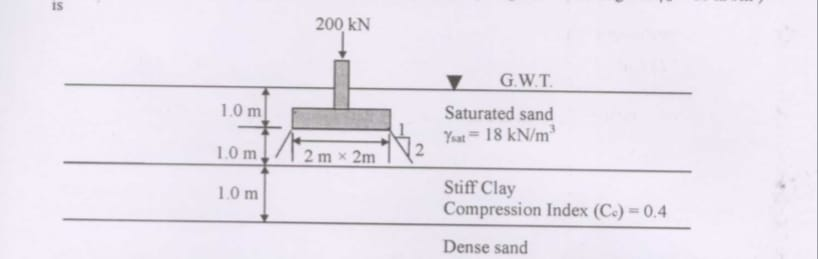
\includegraphics[width=0.7\columnwidth]{figs/image7.jpg}
    \caption{}
    \label{fig:placeholder}
    \end{figure}
    
    \begin{multicols}{2}
    \begin{enumerate}
        \item 32.78 mm 
        \item 61.75 mm 
        \item 79.5 mm 
        \item 131.13 mm
    \end{enumerate}
\end{multicols}
\end{enumerate}

\end{document}
